\documentclass[
  bibliography=totoc,     % Literatur im Inhaltsverzeichnis
  captions=tableheading,  % Tabellenüberschriften
  titlepage=firstiscover, % Titelseite ist Deckblatt
]{scrartcl}

% Paket float verbessern
\usepackage{scrhack}

% Warnung, falls nochmal kompiliert werden muss
\usepackage[aux]{rerunfilecheck}

% unverzichtbare Mathe-Befehle
\usepackage{amsmath}
% viele Mathe-Symbole
\usepackage{amssymb}
% Erweiterungen für amsmath
\usepackage{mathtools}

% Fonteinstellungen
\usepackage{fontspec}
% Latin Modern Fonts werden automatisch geladen
% Alternativ zum Beispiel:
%\setromanfont{Libertinus Serif}
%\setsansfont{Libertinus Sans}
%\setmonofont{Libertinus Mono}

% Wenn man andere Schriftarten gesetzt hat,
% sollte man das Seiten-Layout neu berechnen lassen
\recalctypearea{}

% deutsche Spracheinstellungen
\usepackage[ngerman]{babel}


\usepackage[
  math-style=ISO,    % ┐
  bold-style=ISO,    % │
  sans-style=italic, % │ ISO-Standard folgen
  nabla=upright,     % │
  partial=upright,   % │
  mathrm=sym,        % ┘
  warnings-off={           % ┐
    mathtools-colon,       % │ unnötige Warnungen ausschalten
    mathtools-overbracket, % │
  },                       % ┘
]{unicode-math}

% traditionelle Fonts für Mathematik
\setmathfont{Latin Modern Math}
% Alternativ zum Beispiel:
%\setmathfont{Libertinus Math}

\setmathfont{XITS Math}[range={scr, bfscr}]
\setmathfont{XITS Math}[range={cal, bfcal}, StylisticSet=1]

% Zahlen und Einheiten
\usepackage[
  locale=DE,                   % deutsche Einstellungen
  separate-uncertainty=true,   % immer Unsicherheit mit \pm
  per-mode=symbol-or-fraction, % / in inline math, fraction in display math
]{siunitx}

% chemische Formeln
\usepackage[
  version=4,
  math-greek=default, % ┐ mit unicode-math zusammenarbeiten
  text-greek=default, % ┘
]{mhchem}

% richtige Anführungszeichen
\usepackage[autostyle]{csquotes}

% schöne Brüche im Text
\usepackage{xfrac}

% Standardplatzierung für Floats einstellen
\usepackage{float}
\floatplacement{figure}{htbp}
\floatplacement{table}{htbp}

% Floats innerhalb einer Section halten
\usepackage[
  section, % Floats innerhalb der Section halten
  below,   % unterhalb der Section aber auf der selben Seite ist ok
]{placeins}

% Seite drehen für breite Tabellen: landscape Umgebung
\usepackage{pdflscape}

% Captions schöner machen.
\usepackage[
  labelfont=bf,        % Tabelle x: Abbildung y: ist jetzt fett
  font=small,          % Schrift etwas kleiner als Dokument
  width=0.9\textwidth, % maximale Breite einer Caption schmaler
]{caption}
% subfigure, subtable, subref
\usepackage{subcaption}

% Grafiken können eingebunden werden
\usepackage{graphicx}

% schöne Tabellen
\usepackage{tabularray}
\UseTblrLibrary{booktabs, siunitx}

% Verbesserungen am Schriftbild
\usepackage{microtype}

% Literaturverzeichnis
\usepackage[
  backend=biber,
]{biblatex}
% Quellendatenbank
\addbibresource{lit.bib}
\addbibresource{programme.bib}

% Hyperlinks im Dokument
\usepackage[
  german,
  unicode,        % Unicode in PDF-Attributen erlauben
  pdfusetitle,    % Titel, Autoren und Datum als PDF-Attribute
  pdfcreator={},  % ┐ PDF-Attribute säubern
  pdfproducer={}, % ┘
]{hyperref}
% erweiterte Bookmarks im PDF
\usepackage{bookmark}

% Trennung von Wörtern mit Strichen
\usepackage[shortcuts]{extdash}

\author{%
  Vincent Wirsdörfer\\%
  \href{mailto:vincent.wirsdoerfer@udo.edu}{authorA@udo.edu}%
  \and%
  Joris Daus\\%
  \href{mailto:joris.daus@udo.edu}{authorB@udo.edu}%
}
\publishers{TU Dortmund – Fakultät Physik}


\begin{document}

\section{Zielsetzung}
\label{sec:Zielsetzung}

Das Ziel des im folgend protokollierten Versuchs besteht darin, die Strom- Spannungskennlinie einer Photozelle aufzunehmen. Zusätzlich soll das \emph{Plancksche
Wirkungsquantum}, eine fundamentale Naturkonstante, über die Gegenfeldmethode ermittelt werden.

\section{Theorie}
\label{sec:Theorie}

Das grundlegende Prinzip des Photoeffekts ist die Emission bzw. das Herauslösen von Elektronen aus einem Material aufgrund von Lichteinwirkung. Über den äußeren 
Lichtelektrischen Effekt soll im Folgenden die Plancksche Konstante $h$ bestimmt werden. Diese beschreibt den wesentlichen Zusammehang zwischen Strahlungsenergie
$E_\gamma$ und der Frequenz $f$ über die Gleichung 

\begin{equation*}
    E_\gamma = hf.
\end{equation*}

\noindent Das Prdoukt $hf$ ist dabei Ausdruck für die Interpratation des Photons als gequanteltes Energiepaket. Dies impliziert bereits, dass diverse Phänomene des 
Photoeffekts nicht vollständig durch die klassische Wellentheorie des Lichts erklärt werden können. Einerseits kann die Beobachtung, dass die abgestrahlte Lichtintensität 
proportional zur Anzahl der von der Oberfläche herausgelösten Elektronen ist, gut von der Theorie von Licht als elektromagnetische Welle erklärbar. 
Andererseits ist der instantane Einsatz eines Photostroms mit der Bestrahlung des Materials, die materialabhängige Grenzfrequenz und die Frequenzabhängigkeit der 
kinetischen Energie nicht mit dem Formalismus der Wellentheorie vereinbar.\\

\noindent Beobachet werden hier ausschließlich Metalle, welche im Kern aus positiven Ionenrümpfen bestehen, die von frei beweglichen Elektronen umgeben sind. Energetisch
beschrieben werden die Elektronen durch eine \emph{Fermi-Dirac-Verteilung}. Diese gibt an, mit welcher Wahrscheinlickkeit sich ein Zustand mit Energie $E$ im thermischen 
Gleichgewicht befindet. Visualisiert wird diese Verteilung in der untenstehenden Abbildung.

\begin{figure}
    \centering
    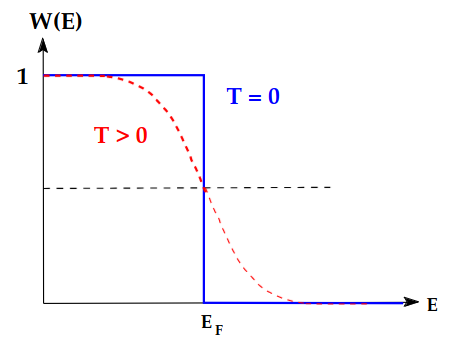
\includegraphics[height=5cm]{FDV.png}
    \caption{Fermi-Dirac-Verteilung\cite{Versuchsanleitung_v500}.}
    \label{fig:FDV}
\end{figure}

\noindent Bei einer Temperatur von $T = \qty{0}{\kelvin}$ sind somit alle Zustände unterhalb der Fermi-Energie $E_\text{F}$ besetzt. Sowohl über- als auch unterhalb 
von $E_\text{F}$ befinden sich die Zustände bei einer Systempräparation von $T > \qty{0}{\kelvin}$. Daher muss zusätzliche Energie aufgewendet werden, um ein Elektron 
aus dem Metall zu lösen. Die dafür benötigte Energie wird als \emph{Austrittsarbeit} bezeichnet. Die hier betrachtete Energiezufuhr erfolgt mittels elektromagnetischer 
Strahlung mit Energie $E_\gamma = hf$. Ist diese Enerie gleich der Austrittsarbeit, so werden Elektronen herausgelöst. Bei noch größeren Energiemengen, wird die
überschüssige Energie oberhalb der Austrittsarbeit $\Phi$ in Form von kinetischer Energie an das Elektron abgegeben:

\begin{equation}
    E_\gamma = \Phi + \frac{1}{2}mv²
\label{eqn:Energiebilanz1}
\end{equation}

\noindent Um einen konkreteren Ausdruck für die kinetische Energie der Elektronen zu erhalten, wird die Gegenfeldmethode angewendet. Diese funktionert folgenderweise.
Gegenüber der Photokathode befindet sich eine Anode, welche durch Anlegen einer Spannung ein elektrisches Feld erzeugt. Dieses Feld kann je nach Vorzeichen der Spannung 
die aus der Kathode emitierten Elektronen beschleunigen oder abbremsen. Im Falle einer Abbremsung kann die Spannung so angepasst werde, sodass die Elektronen gerade nicht 
die Anode erreichen. Die dafür benötigte Spannung wird \emph{Grenzspannung} $U_\text{G}$ tituliert. Aus der Energieäquivalenz $E_\text{kin} =  E_\text{el}$ kann somit die 
Energiebilanz aus \eqref{eqn:Energiebilanz1} umgeschrieben werden als 

\begin{equation}
    E_\gamma = hf = \Phi + eU_\text{G},
\label{eqn:Energiebilanz2}
\end{equation}

\noindent wobei $\Phi = hf_\text{G}$ die Austrittsarbeit mit $f_\text{G}$ als Grenzfrequenz bezeichnet. Eine Darstellung dieser Idee liefert die folgende Abbildung.

\begin{figure}
    \centering
    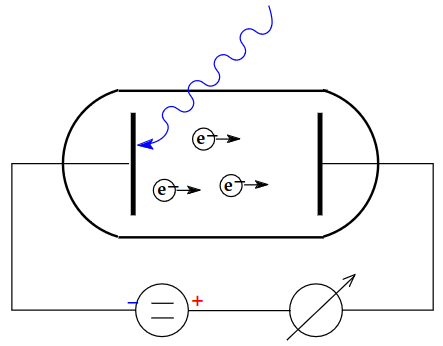
\includegraphics[height=5cm]{Gegenfeldmethode.png}
    \caption{Gegenfeldmethode zur Ermittlung des Planck'schen Wirkungsquantumm\cite{Versuchsanleitung_v500}.}
    \label{fig:Gegenfeldmethode}
\end{figure}

%\section{Vorbereitung}

%\section{Fehlerrechnung}
\end{document}